\documentclass{beamer}
\usepackage{graphicx}
\usepackage{xcolor}
\usepackage{tikz}
\usepackage{amsmath}
\usepackage{pgfplots}
\pgfplotsset{compat=1.18}

% 自定义颜色
\definecolor{purpleblue}{RGB}{80, 80, 180}
\definecolor{lightgray}{RGB}{230, 230, 230}
\definecolor{novelPurple}{RGB}{98, 54, 255}
\definecolor{darkgray}{RGB}{50, 50, 50}
\definecolor{softPurple}{RGB}{180, 170, 255}
\definecolor{softGray}{RGB}{235, 235, 245}
\definecolor{lightText}{RGB}{90, 90, 110}
\graphicspath{{static/course_materials/}{./}}

% 主题设置
\usetheme{Madrid}
\usecolortheme{dolphin}

\setbeamerfont{title}{size=\Large,series=\bfseries}
\setbeamerfont{frametitle}{size=\LARGE,series=\bfseries}
\setbeamercolor{frametitle}{fg=white, bg=novelPurple}
\setbeamercolor{title}{fg=white, bg=purpleblue}

\title[SAT Unit 3.4]{\textbf{SAT Unit 3.4 \\Models and Scatterplots}}
\author{\textbf{Jack Zeng}}
\institute{\textcolor{white}{\textbf{Novel Prep}}}
\date{\today}

\begin{document}


% --- Title Slide ---
\begin{frame}
    \titlepage
    \vfill
    \begin{flushright}
        \textcolor{purpleblue}{\Huge \textbf{Novel Prep}}
    \end{flushright}
\end{frame}

\begin{frame}
    \begin{tikzpicture}[remember picture, overlay]
        \shade[top color=softPurple, bottom color=softGray]
            (current page.north west) rectangle (current page.south east);
        \fill[white, opacity=0.3] (current page.center) circle (4cm);
        \node[align=center] at (current page.center) {
            {\Huge\bfseries\textcolor{purpleblue}{Novel Prep}} \\[0.5cm]
            {\Large\itshape\textcolor{lightText}{Excellence in SAT Prep}}
        };
        \foreach \x in {1,2,3,4,5} {
            \fill[purpleblue, opacity=0.2] (rand*10-5, rand*7-3.5) circle (0.1+\x*0.05);
        }
    \end{tikzpicture}
\end{frame}

\begin{frame}{Overview}
    \tableofcontents
\end{frame}

\begin{frame}
\section{Linear vs Exponential Model}
    \begin{tikzpicture}[remember picture, overlay]
        % 设置浅色渐变背景
        \shade[top color=softPurple, bottom color=softGray] 
            (current page.north west) rectangle (current page.south east);
        
        % 添加高斯模糊光晕
        \fill[white, opacity=0.3] (current page.center) circle (4cm);
        
        % 主标题
        \node[align=center] at (current page.center) {
            {\LARGE\bfseries\textcolor{purpleblue}{ Linear vs Exponential Model}} \\[0.5cm]
            {\Large\itshape\textcolor{lightText}{Excellence in SAT Prep}}
        };

        % 添加柔和光点（点缀）
        \foreach \x in {1,2,3,4,5} {
            \fill[purpleblue, opacity=0.2] (rand*10-5, rand*7-3.5) circle (0.1+\x*0.05);
        }

        ;
    \end{tikzpicture}
\end{frame}

\begin{frame}{Linear Models}
    
\textbf{Definition:}  
A linear model shows a \textbf{constant rate of change} — the dependent variable increases or decreases by the same amount for every unit increase in the independent variable.

\[
y = mx + b
\]

\textbf{Where:}
\begin{itemize}
    \item \(m\) is the slope (rate of change)
    \item \(b\) is the \(y\)-intercept (starting value)
\end{itemize}

\textbf{Key Characteristics:}
\begin{itemize}
    \item Graph is a straight line.
    \item Change is additive.
    \item Example: Earning \$15/hour → \(y = 15x\)
\end{itemize}

\end{frame}


\begin{frame}{Exponential Models}
    
\textbf{Definition:}  
An exponential model shows a \textbf{constant percentage rate of change} — the quantity increases or decreases by the same \textbf{proportion} over equal intervals.

\[
y = a \cdot b^x
\]

\textbf{Where:}
\begin{itemize}
    \item \(a\) is the initial value
    \item \(b\) is the growth (\(b > 1\)) or decay (\(0 < b < 1\)) factor
\end{itemize}

\textbf{Key Characteristics:}
\begin{itemize}
    \item Graph is curved — increasing/decreasing rapidly.
    \item Change is multiplicative.
    \item Example: Population doubles each hour → \(y = 100 \cdot 2^x\)
\end{itemize}
\end{frame}

\begin{frame}{\textbf{Exponential Decay – Interpretation of Parameters}}
\textbf{Question:} 

The function \( M(t) = 4000(0.6)^{\frac{t}{3}} \) models the mass, in nanograms, of a particle after \( t \) years. 

Which of the following is the best interpretation of \( (0.6)^{\frac{t}{3}} \) in this context?

\begin{itemize}
    \item[\textbf{A.}] The mass of the particle decreases by 60\% every 4 months.
    \item[\textbf{B.}] The mass of the particle decreases by 60\% every 3 years.
    \item[\textbf{C.}] The mass of the particle decreases by 40\% every 4 months.
    \item[\textbf{D.}] The mass of the particle decreases by 40\% every 3 years.
\end{itemize}
\end{frame}

\begin{frame}{\textbf{Answer: Decay Rate over Time}}
\textbf{Explanation:}

The exponential function is of the form:
\[
M(t) = 4000 \cdot (0.6)^{\frac{t}{3}},
\]
which means that every 3 years, the mass is multiplied by 0.6 — a 40\% decrease from the previous amount.

\textbf{Correct Answer:} \( \boxed{D} \)
\end{frame}




\begin{frame}{Comparing Linear vs Exponential Models}
    
\textbf{Linear:} Constant difference  
\textbf{Exponential:} Constant ratio

\vspace{0.3cm}
\begin{tabular}{|l|c|c|}
\hline
\textbf{Feature} & \textbf{Linear} & \textbf{Exponential} \\
\hline
\textbf{General Form} & \(y = mx + b\) & \(y = a \cdot b^x\) \\
\textbf{Rate of Change} & Constant (add/subtract) & Constant (multiply/divide) \\
\textbf{Graph Shape} & Straight line & Curve (growth/decay) \\
\textbf{Example} & \$10 per day & Double each day \\
\textbf{Real-World Use} & Salaries, fees & Populations, investments \\
\hline
\end{tabular}

\vspace{0.3cm}
\textbf{Key Insight:}  
If the rate of change is constant \textbf{difference}, it's linear.  
If the rate of change is constant \textbf{ratio}, it's exponential.

\end{frame}



\begin{frame}{\textbf{Question: Linear Functions – Percentage Relationship}}
For \( x > 0 \), the function \( f \) is defined as follows: \( f(x) \) equals \( 201\% \) of \( x \).

Which of the following could describe this function?

\begin{itemize}
    \item[\textbf{A.}] Decreasing exponential
    \item[\textbf{B.}] Decreasing linear
    \item[\textbf{C.}] Increasing exponential
    \item[\textbf{D.}] Increasing linear
\end{itemize}
\end{frame}

\begin{frame}{\textbf{Answer Explanation: Linear Functions – Percentage Relationship}}
Since \( 201\% \) of \( x \) means \( f(x) = 2.01x \), this is a linear function with a positive slope, so it increases at a constant rate.

\textbf{Correct Answer:} \( \boxed{D} \)
\end{frame}

\begin{frame}{Practice: Identify the Model Type}
    
\textbf{A population of bacteria is observed to grow as follows:}

\begin{center}
\begin{tabular}{|c|c|}
\hline
\textbf{Time (hours)} & \textbf{Population} \\
\hline
0 & 100 \\
1 & 200 \\
2 & 400 \\
3 & 800 \\
\hline
\end{tabular}
\end{center}

\vspace{0.2cm}
\textbf{Question:}  
Which type of model best describes this data?

\begin{itemize}
    \item[\textbf{A.}] Linear Model
    \item[\textbf{B.}] Exponential Model
    \item[\textbf{C.}] Neither
\end{itemize}

\end{frame}

\begin{frame}{\textbf{Answer Explanation: Identify the Model Type}}
The population doubles each hour: \(100 \rightarrow 200 \rightarrow 400 \rightarrow 800\). This shows a \textbf{constant ratio} (multiply by 2), so the model is \( P(t) = 100 \cdot 2^t \).

\textbf{Correct Answer:} \( \boxed{B} \)
\end{frame}


\begin{frame}
\section{Scatterplots and Regression}
    \begin{tikzpicture}[remember picture, overlay]
        % 设置浅色渐变背景
        \shade[top color=softPurple, bottom color=softGray] 
            (current page.north west) rectangle (current page.south east);
        
        % 添加高斯模糊光晕
        \fill[white, opacity=0.3] (current page.center) circle (4cm);
        
        % 主标题
        \node[align=center] at (current page.center) {
            {\LARGE\bfseries\textcolor{purpleblue}{ Scatterplots and Regression}} \\[0.5cm]
            {\Large\itshape\textcolor{lightText}{Excellence in SAT Prep}}
        };

        % 添加柔和光点（点缀）
        \foreach \x in {1,2,3,4,5} {
            \fill[purpleblue, opacity=0.2] (rand*10-5, rand*7-3.5) circle (0.1+\x*0.05);
        }

        ;
    \end{tikzpicture}
\end{frame}

\begin{frame}{Understanding Scatterplots}
    
\textbf{Definition:}  
A \textbf{scatterplot} is a graph that displays pairs of data points \((x, y)\) as dots in the coordinate plane.

\vspace{0.3cm}
\textbf{Purpose:}
\begin{itemize}
    \item Visualizes the relationship between two numerical variables.
    \item Reveals trends, clusters, outliers, or correlation direction.
\end{itemize}

\vspace{0.3cm}
\textbf{Types of Trends:}
\begin{itemize}
    \item \textbf{Positive association:} As \(x\) increases, \(y\) increases.
    \item \textbf{Negative association:} As \(x\) increases, \(y\) decreases.
    \item \textbf{No association:} No visible pattern or relationship.
\end{itemize}

\vspace{0.3cm}
\textbf{Note:} Scatterplots do not imply causation, only correlation.

\end{frame}

\begin{frame}{Scatterplots and Linear Regression}

\begin{center}
    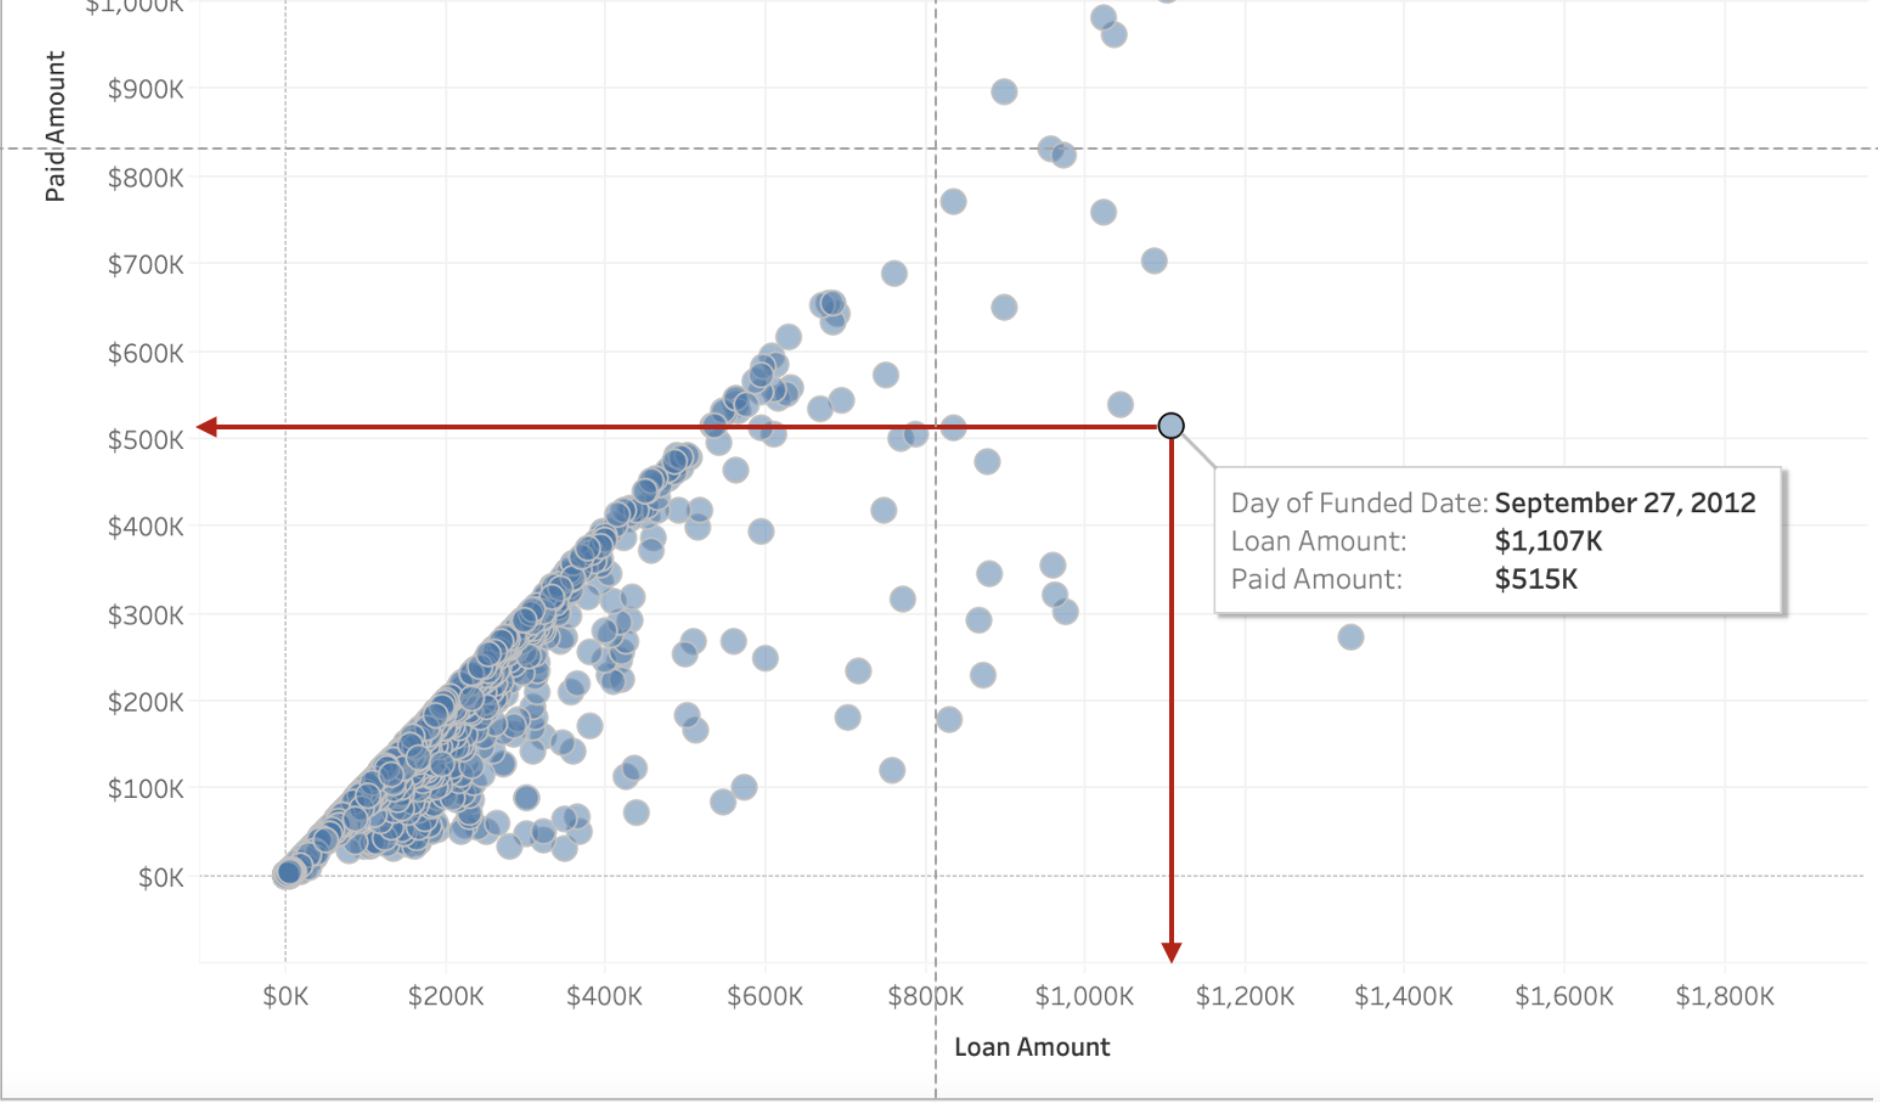
\includegraphics[width=0.72\linewidth]{E33.png}
\end{center}

\vspace{-0.15cm}
\textbf{Linear regression} is a line of best fit through a scatterplot: \( y = mx + b \), where \( m \) is slope and \( b \) is the \( y \)-intercept. It minimizes squared vertical distances (residuals) and is used for prediction. The closer the points are to the line, the stronger the linear relationship.

\end{frame}


\begin{frame}{\textbf{Question: Line of Best Fit from Scatterplot}}

\begin{center}
    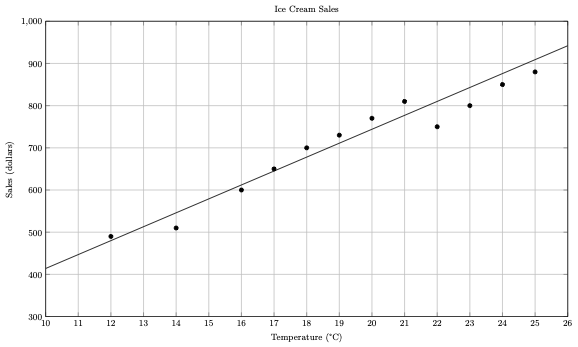
\includegraphics[width=0.48\linewidth]{E34.png}
\end{center}

\vspace{-0.2cm}
\small
The scatterplot above shows a company's ice cream sales \( d \), in dollars, and the high temperature \( t \), in degrees Celsius (°C), on 12 different days. A line of best fit for the data is also shown.

Which of the following could be an equation of the line of best fit?

\begin{itemize}
    \item[\textbf{A.}] \( d = 0.03t + 402 \)
    \item[\textbf{B.}] \( d = 10t + 402 \)
    \item[\textbf{C.}] \( d = 33t + 300 \)
    \item[\textbf{D.}] \( d = 33t + 84 \)
\end{itemize}


\end{frame}


\begin{frame}{\textbf{Answer Explanation: Line of Best Fit from Scatterplot}}
From the scatterplot:
\begin{itemize}
    \item The line of best fit passes through approximately \( (12, 480) \) and \( (24, 876) \)
    \item Estimating the slope:
    \[
    \text{slope} = \frac{876 - 480}{24 - 12} = \frac{396}{12} = 33
    \]
    \item Plug into point-slope form:
    \[
    d - 480 = 33(t - 12) \Rightarrow d = 33t + 84
    \]
\end{itemize}

\textbf{Correct Answer:} \( \boxed{D} \)
\end{frame}


\begin{frame}
\section{Practice}
    \begin{tikzpicture}[remember picture, overlay]
        % 设置浅色渐变背景
        \shade[top color=softPurple, bottom color=softGray] 
            (current page.north west) rectangle (current page.south east);
        
        % 添加高斯模糊光晕
        \fill[white, opacity=0.3] (current page.center) circle (4cm);
        
        % 主标题
        \node[align=center] at (current page.center) {
            {\LARGE\bfseries\textcolor{purpleblue}{ Practices}} \\[0.5cm]
            {\Large\itshape\textcolor{lightText}{Excellence in SAT Prep}}
        };

        % 添加柔和光点（点缀）
        \foreach \x in {1,2,3,4,5} {
            \fill[purpleblue, opacity=0.2] (rand*10-5, rand*7-3.5) circle (0.1+\x*0.05);
        }

        ;
    \end{tikzpicture}
\end{frame}

\begin{frame}{\textbf{Question: Slope of Line of Best Fit}}

\begin{center}
    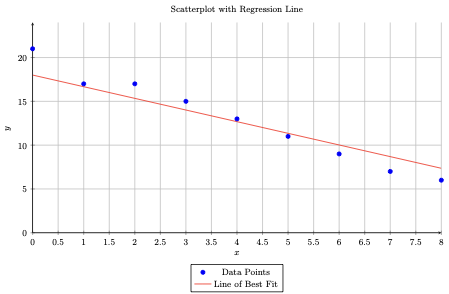
\includegraphics[width=0.55\linewidth]{E35.png}
\end{center}

Which of the following is closest to the slope of the line of best fit shown?

\begin{itemize}
 \item[\textbf{A.}] \(-2.16\)
 \item[\textbf{B.}] \(-1.38\)
 \item[\textbf{C.}] \(-0.72\)
 \item[\textbf{D.}] \(-0.46\)
\end{itemize}
\end{frame}


\begin{frame}{\textbf{Answer Explanation: Which of the following is closest to the slope of the…}}
\textbf{Step 1. Find two points on the line of best fit:}
\begin{itemize}
    \item At \(x=1\), \(y \approx 17\).
    \item At \(x=4\), \(y \approx 13\).
\end{itemize}

\textbf{Step 2. Compute the slope:}
\[
\text{slope} = \frac{13-17}{4 - 1} = \frac{-4}{3} \approx -1.33.
\]

\textbf{Step 3. Choose the closest answer:}
\[
-1.33 \text{ is closest to } -1.38.
\]

\textbf{Correct Answer:} \( \boxed{B} \)
\end{frame}



\begin{frame}{\textbf{Question: An online service currently has 8,400 users. A random…}}
An online service currently has 8,400 users. A random sample of 350 users was selected and asked whether they will renew their subscription to the service. Of those surveyed, 12\% stated that they will not renew their subscription. Based on this survey, which of the following is the best estimate of the total number of users who will not renew their subscription?

\begin{itemize}
 \item[\textbf{A.}] 42
 \item[\textbf{B.}] 200
 \item[\textbf{C.}] 1,008
 \item[\textbf{D.}] 7,392
\end{itemize}
\end{frame}


\begin{frame}{\textbf{Answer Explanation: An online service currently has 8,400 users. A random…}}
\textbf{Step 1. Calculate the estimated percentage of non-renewing users:}
\[
0.12 \times 8,400 = 1,008.
\]

\textbf{Correct Answer:} \( \boxed{C} \)
\end{frame}


\begin{frame}{\textbf{Question: The employees at a new bookstore must stock a certain…}}
The employees at a new bookstore must stock a certain number of shelves so that the store is ready for its opening in two weeks. The employees stock shelves at a constant rate throughout the two weeks. If \(p(t)\) is the number of shelves left to be stocked after \(t\) days, which of the following statements best describes the function \(p\)?

\begin{itemize}
 \item[\textbf{A.}] The function \(p\) is an increasing exponential function.
 \item[\textbf{B.}] The function \(p\) is a decreasing exponential function.
 \item[\textbf{C.}] The function \(p\) is an increasing linear function.
 \item[\textbf{D.}] The function \(p\) is a decreasing linear function.
\end{itemize}
\end{frame}


\begin{frame}{\textbf{Answer Explanation: The employees at a new bookstore must stock a certain…}}
\textbf{Step 1.} Since shelves are stocked at a constant rate, the rate of decrease in the number of shelves left to stock is constant. That means \(p(t)\) is decreasing linearly.

\textbf{Correct Answer:} \( \boxed{D} \)
\end{frame}


\begin{frame}{\textbf{Question: For the function \(f\), the value of \(f(x)\) is equal…}}
For the function \(f\), the value of \(f(x)\) is equal to half the value of \(x\). Which of the following is the best description of this function?

\begin{itemize}
 \item[\textbf{A.}] Decreasing linear
 \item[\textbf{B.}] Decreasing exponential
 \item[\textbf{C.}] Increasing linear
 \item[\textbf{D.}] Increasing exponential
\end{itemize}
\end{frame}



\begin{frame}{\textbf{Answer Explanation: For the function \(f\), the value of \(f(x)\) is equal…}}
\textbf{Step 1.} The function is \(f(x) = \frac{1}{2}x\).

\textbf{Step 2.} Since the function is a constant multiple of \(x\), it is a linear function.

\textbf{Step 3.} The coefficient \(\frac{1}{2}\) is positive, so the function is increasing.

\textbf{Correct Answer:} \( \boxed{C} \)
\end{frame}

\begin{frame}{}
    \begin{tikzpicture}[remember picture, overlay]
        \shade[top color=novelPurple!40, bottom color=white]
            (current page.north west) rectangle (current page.south east);
        \fill[white, opacity=0.15] (current page.center) circle (5cm);
        \foreach \x in {1,2,3,4,5} {
            \fill[novelPurple, opacity=0.12] (rand*10-5, rand*7-3.5) circle (0.1+\x*0.05);
        }
    \end{tikzpicture}
    \centering
    \vspace{5em}
    {\Huge \textbf{\textcolor{novelPurple}{Thank You!}}} \\[1em]
    {\large \textcolor{gray}{We appreciate your time and focus.}} \\[3em]
    {\LARGE \textbf{\textcolor{novelPurple}{\textsf{Novel Prep}}}}
    \vfill
\end{frame}

\end{document}
